\documentclass[uplatex,12pt]{jsarticle}
\usepackage[dvipdfmx]{graphicx}
\usepackage{url}
\usepackage{listings,jlisting}
\usepackage{ascmac}
\usepackage{amsmath,amssymb}

%ここからソースコードの表示に関する設定
\lstset{
%  basicstyle={\ttfamily},
  basicstyle={\small},
  identifierstyle={\small},
%  commentstyle={\smallitshape},
%  commentstyle={\small\itshape},
  commentstyle={\small\ttfamily},
  keywordstyle={\small\bfseries},
  ndkeywordstyle={\small},
  stringstyle={\small\ttfamily},
  frame={tb},
  breaklines=true,
  columns=[l]{fullflexible},
  numbers=left,
  xrightmargin=0zw,
  xleftmargin=3zw,
  numberstyle={\scriptsize},
  stepnumber=1,
  numbersep=1zw,
  lineskip=-0.5ex
}
%ここまでソースコードの表示に関する設定

\title{知能プログラミング演習II 課題2}
\author{グループ8\\
  29114060 後藤 拓也\\
}
\date{2019年11月18日}

\begin{document}
\maketitle

\paragraph{提出物} rep4

\paragraph{グループ} グループ8

\paragraph{グループメンバー}
\begin{center}
\begin{tabular}{|c|c|c|}
  \hline
  学生番号&氏名&貢献度比率\\
  \hline\hline
  29114003&青山周平&no\\
  \hline
  29114060&後藤拓也&no\\
  \hline
  29114116&増田大輝&no\\
  \hline
  29114142&湯浅範子&no\\
  \hline
  29119016&小中祐希&no\\
  \hline
\end{tabular}
\end{center}
\paragraph{自分の役割} 必須課題4.2
\\ 「前向き推論,および後ろ向き推論に基づく質問応答システムを作成」
%%%%%%%%%%%%%%%%%%%%%%%%%%%%%%%%%%%%%%%%%%%%%%%%%%%%%%%%%%%%%%%%%%%%%%%%%%%%%%
\section{課題の説明}
\begin{screen}
CarShop.data , AnimalWorld.data 等のデータファイルを実際的な応用事例(自分達の興味分野で良い)に書き換えて,前向き推論,および後ろ向き推論に基づく質問応答システムを作成せよ.どのような応用事例を扱うかは,メンバーで話し合って決めること.
なお,ユーザの質問は英語や日本語のような自然言語が望ましいが,難しければ変数を含むパターン等でも可とする.
\end{screen}

\section{手法}
\begin{enumerate}
\item 後ろ向き推論における英文を用いた質問
\item 前向き推論における英文を用いた質問
\end{enumerate}

\subsection{後ろ向き推論に関して}
後ろ向き推論は, ある仮説を与え, それが現在のアサーション集合において成り立つかをルールを用いて検証していくため, 英語による質問を仮説に当てはめればよい.

ここで問題となるのは, 英語の質問の内容である. 後ろ向き推論はルールの後件部を見て, その前件部がワーキングメモリにあるかとバックトラックしていくので, 質問内容が後件部の内容でない場合は処理されない. 以下に具体例を用いる.

\begin{figure}[htbp]
 \begin{center}
  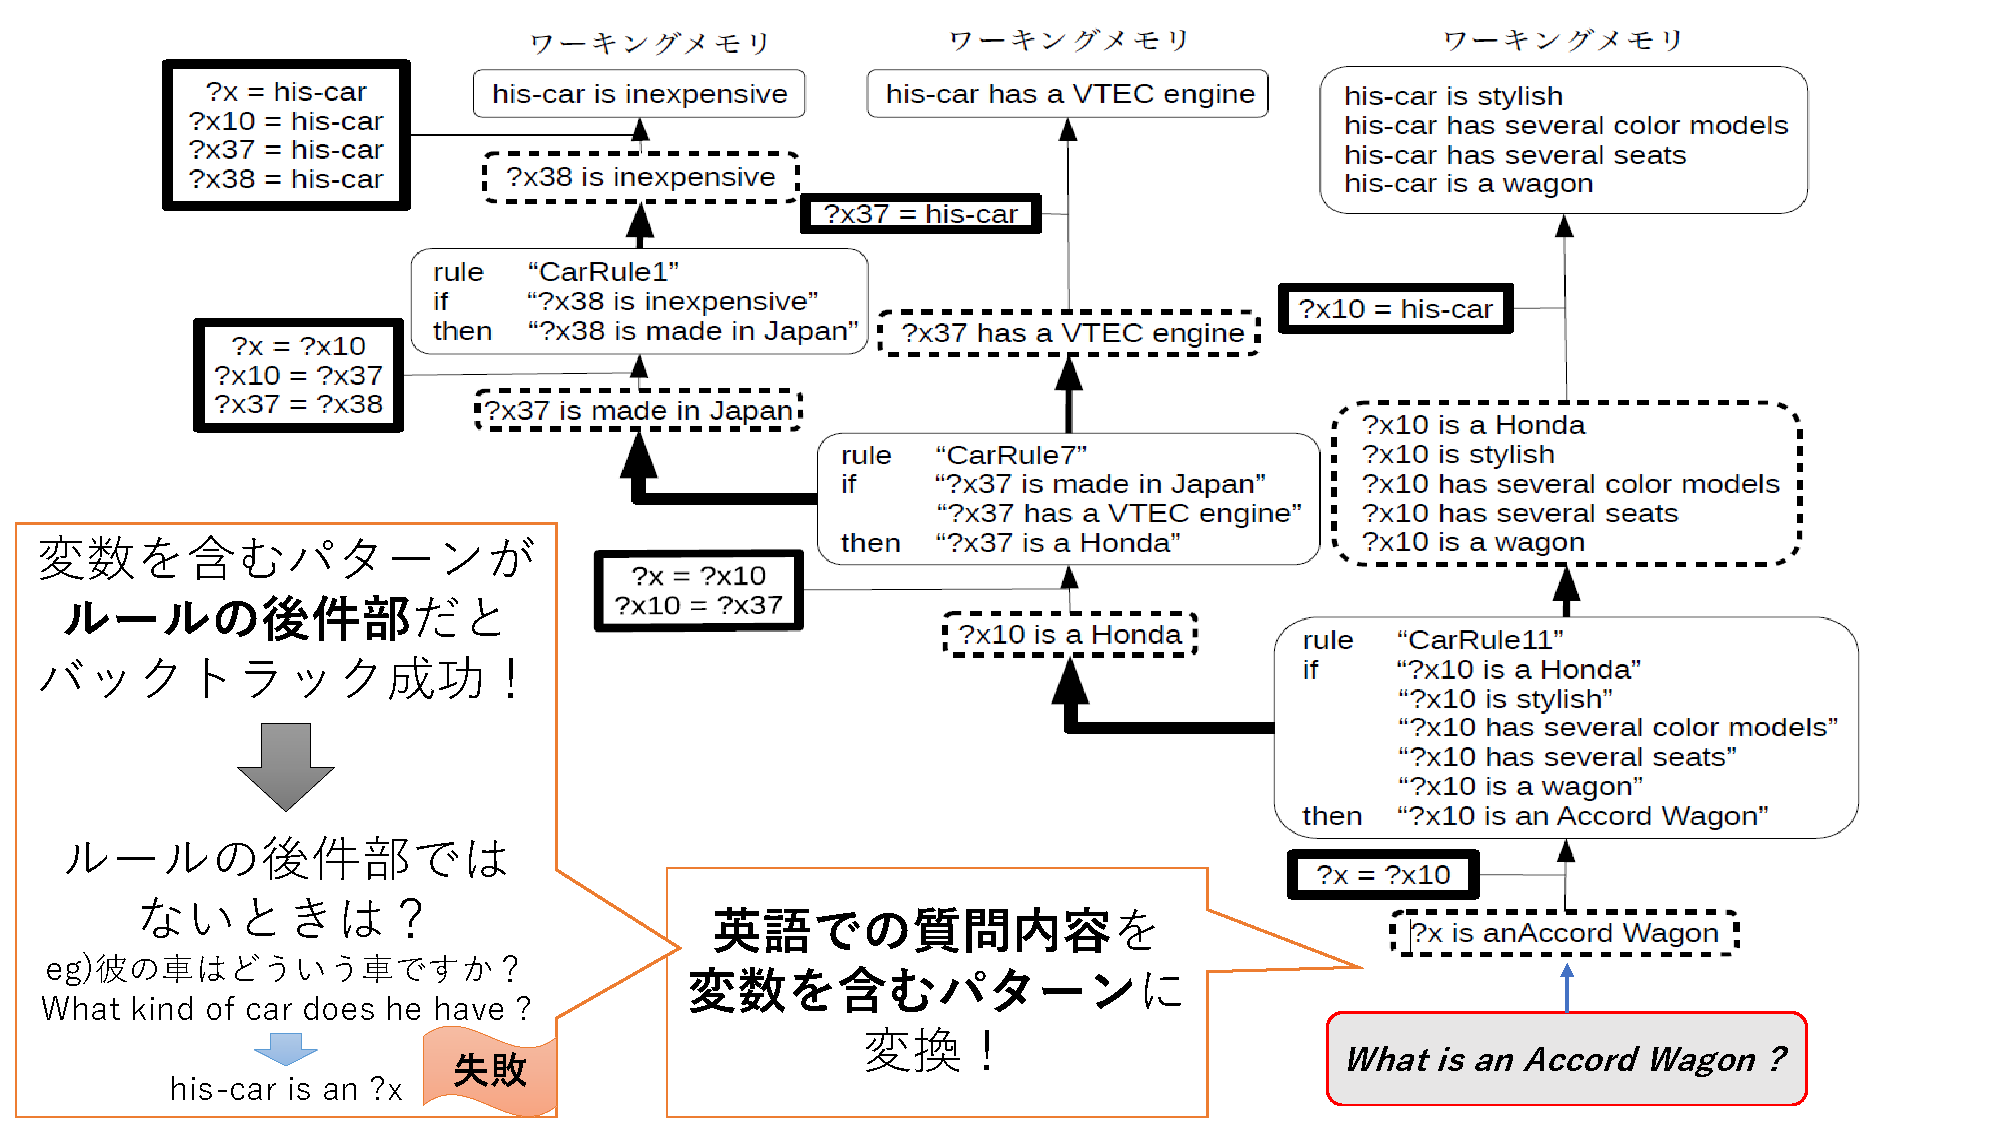
\includegraphics[width = 12cm, pagebox = cropbox, clip]{images/後ろ向き推論_仮説の立て方.pdf}
 \end{center}
 \caption[]{英語の質問を仮説に変換させる}\label{fig:fig1.1}
\end{figure}

質問の内容が「アコードワゴンは何ですか?」と場合, 「?x is an Accord Wagon」に変換でき, それはルールの後件部の内容なので, そのままバックトラックを行えるが, 「彼が持っている車は何ですか?」という場合, 「his-car is ?x」というパターンに変換でき, これはルールの後件部にはないので, バックトラックに失敗する.(正しくは, his-Car is inexpensiveと出力されてしまう.)

また, 質問内容が後件部の内容ではなく, 前件部の内容に関わる内容の場合, ワーキングメモリ内のアサーションを上から照らし合わせていき, 照合するアサーションで出力される. 上記で述べた「his-Car is ?x」も, ワーキングメモリの1番上に「his-Car is inexpensive」が存在するため間違って出力されるのである. また, これらより, 同じ文の形を持っている場合, 1つ目のアサーションにヒットすると, 2つ目まで進まないということも同様に成り立つ. 以下を見てもらいたい.

\begin{figure}[htbp]
 \begin{center}
  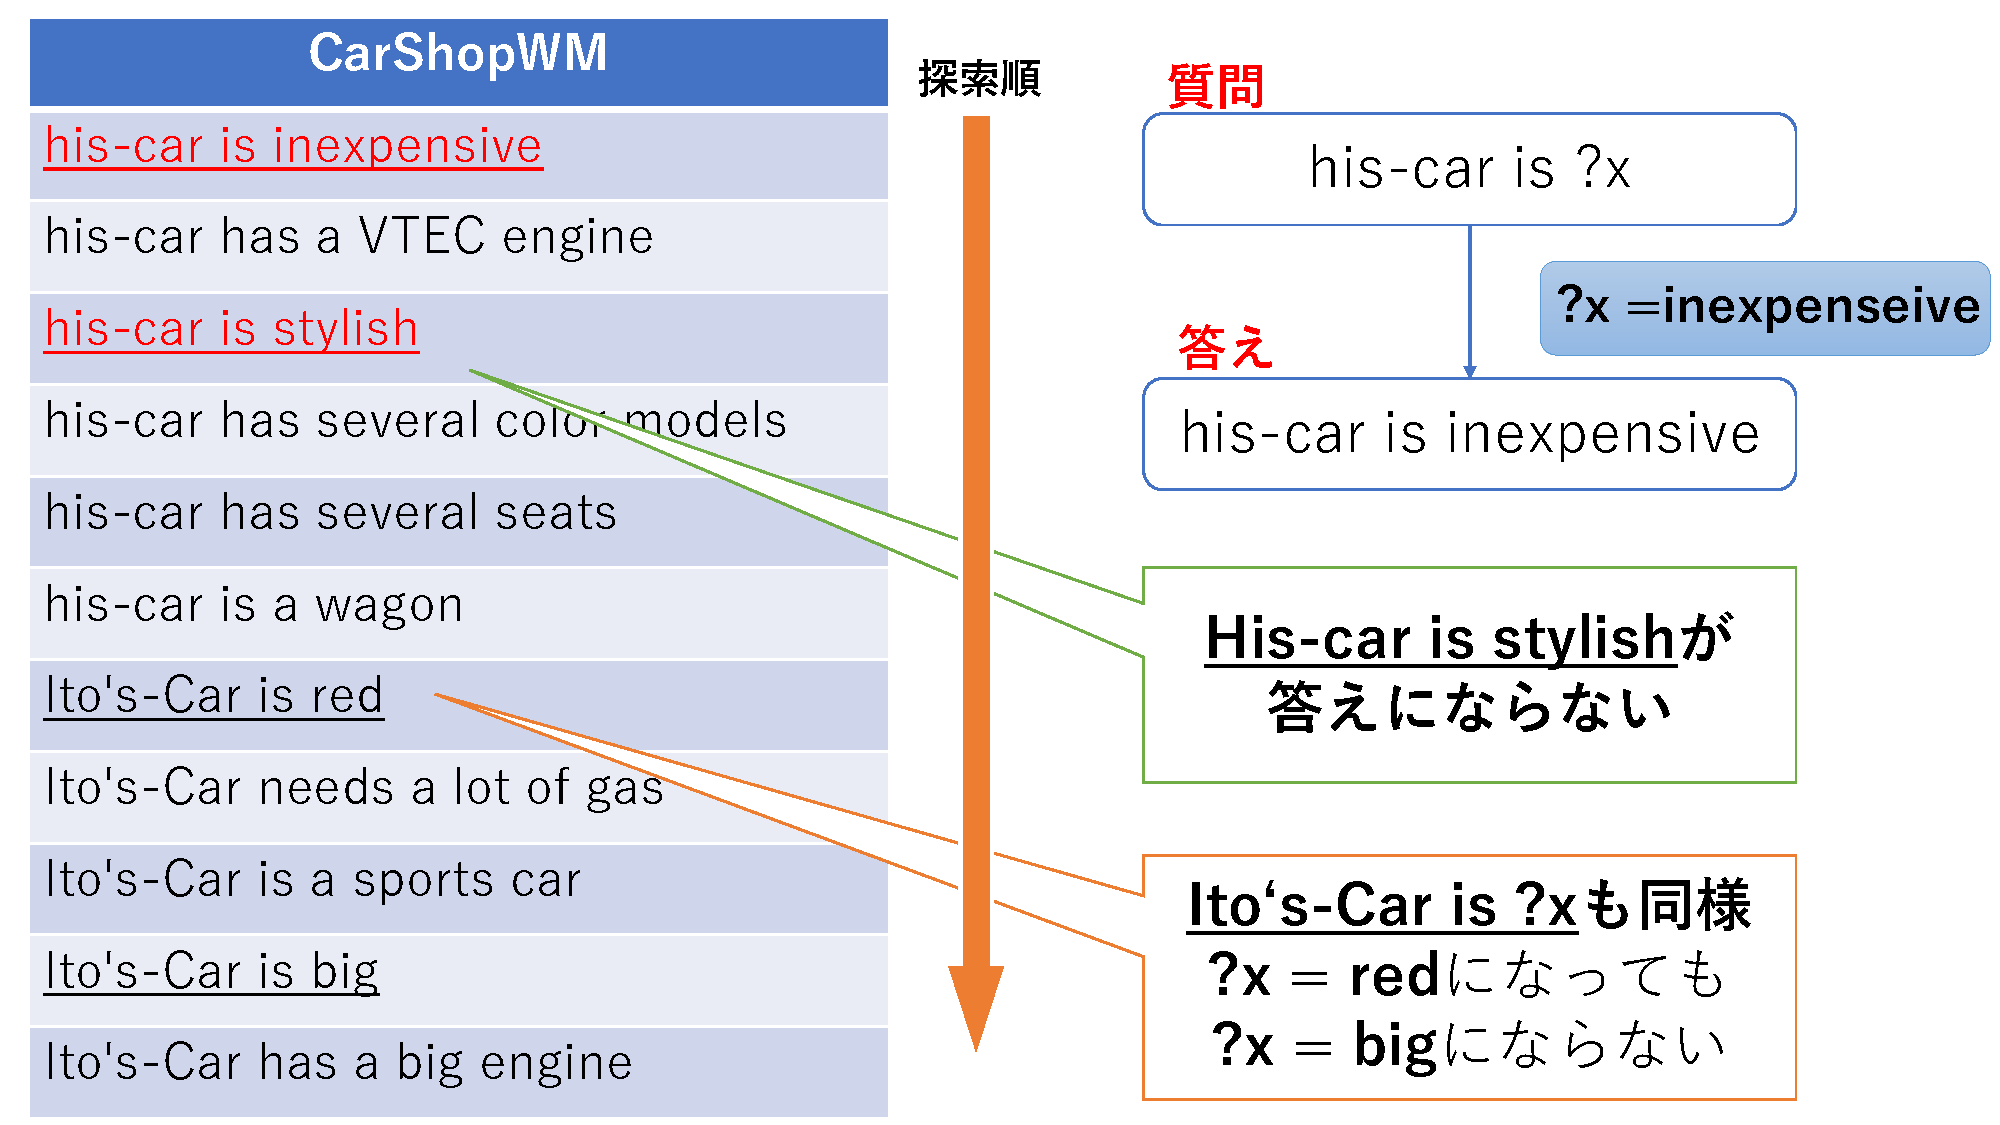
\includegraphics[width = 10cm, pagebox = cropbox, clip]{images/後ろ向き推論_WMの探索.pdf}
 \end{center}
 \caption[]{WM内の探索順序}\label{fig:fig1.1}
\end{figure}

質問の内容によっては, 「his-car is stylish」に基づく内容を問いたくなるだろう. そういった場合, 「his-car is ?x」という形をしているアサーションが複数ある場合に, 何らかの制限を加える必要がある.

ここで, ワーキングメモリにおけるアサーションに対する質問内容を具体化してみる. 「彼の車は安価です.」と「彼の車はスタイリッシュです.」というアサーションが存在する際, 質問とは何であろうか? 「彼の車は安価ですか?」と「彼の車はスタイリッシュですか?」のYes/Noが返事となる質問ではないだろうか? 逆に, 「彼の車は何ですか?」と質問して「彼の車は安価です.」と返ってきたら, むむむと思うのではないだろうか. だが, 「伊藤の車は何色ですか?」と質問したら, 「伊藤の車は赤色です.」と返答がほしい. 

質問内容を, 
\begin{enumerate}
\item Yes/Noで答えることができる質問
\item 具体的な答えを返す質問
\end{enumerate}
に分類した際, 2の"具体的な答えを返す質問"に応えれるように, ワーキングメモリ内のアサーションの並び方や内容など, 工夫する必要がある.

"英語の質問"を"変数を含むパターン"に落とし込む方法は前回の課題のようにクエリーに分けて, 適切に並び替える方法をとる.

\begin{figure}[htbp]
 \begin{center}
  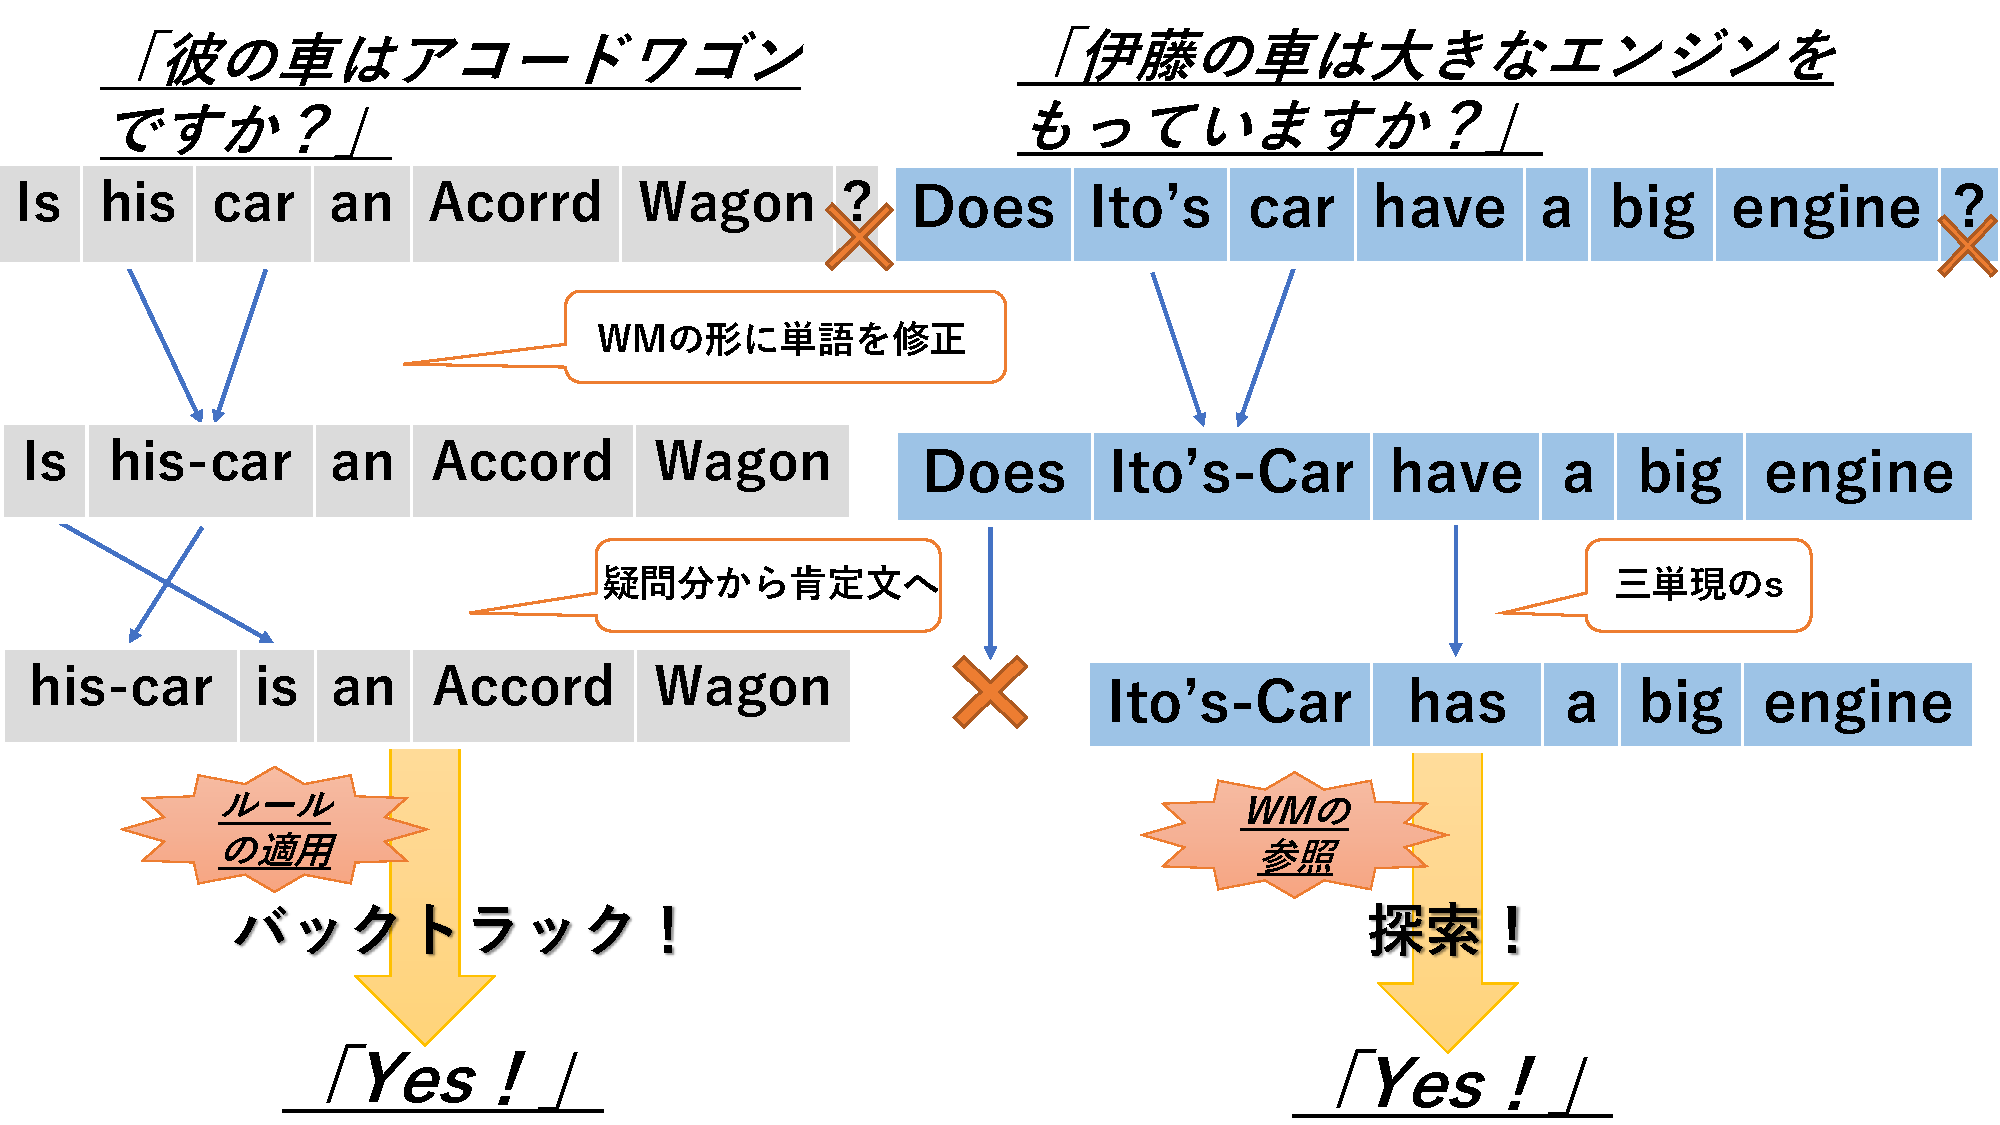
\includegraphics[width = 10cm, pagebox = cropbox, clip]{images/英文構造_YesNo型.pdf}
 \end{center}
 \caption[]{Yes/Noで回答する疑問文の処理}\label{fig:fig1.1}
\end{figure}

疑問分を肯定文に並び変えるのは, SVC構文の場合は, 先頭の2文字を並び替えだけで, SVO構文の場合は, 先頭文字を削除するだけである. 三人称単数の置き換え(haveをhasやneedをneedsなど)など細かい処理もある. 図3における左の例文と右の例文の大きな処理の違いは, 肯定文のパターンに並び変えた後である. 左の例文では, ルールの後件部に該当する内容なので, バックトラックが行われるが, 右の例文では, ルールの後件部には存在しない内容なので, ワーキングメモリを参照される. ワーキングメモリの参照のされ方は, 上記で述べたように, 上から処理される. このYes/Noの答えを返す内容では, この左右の例文に大きな違いは存在しないが, 次の"具体的な答えを返す質問"の際には, これが大きく関わってくる.


具体的な答えを返す質問も似たような処理で英語から変数を含むパターンに落とし込むことができる. 
\begin{figure}[htbp]
 \begin{center}
  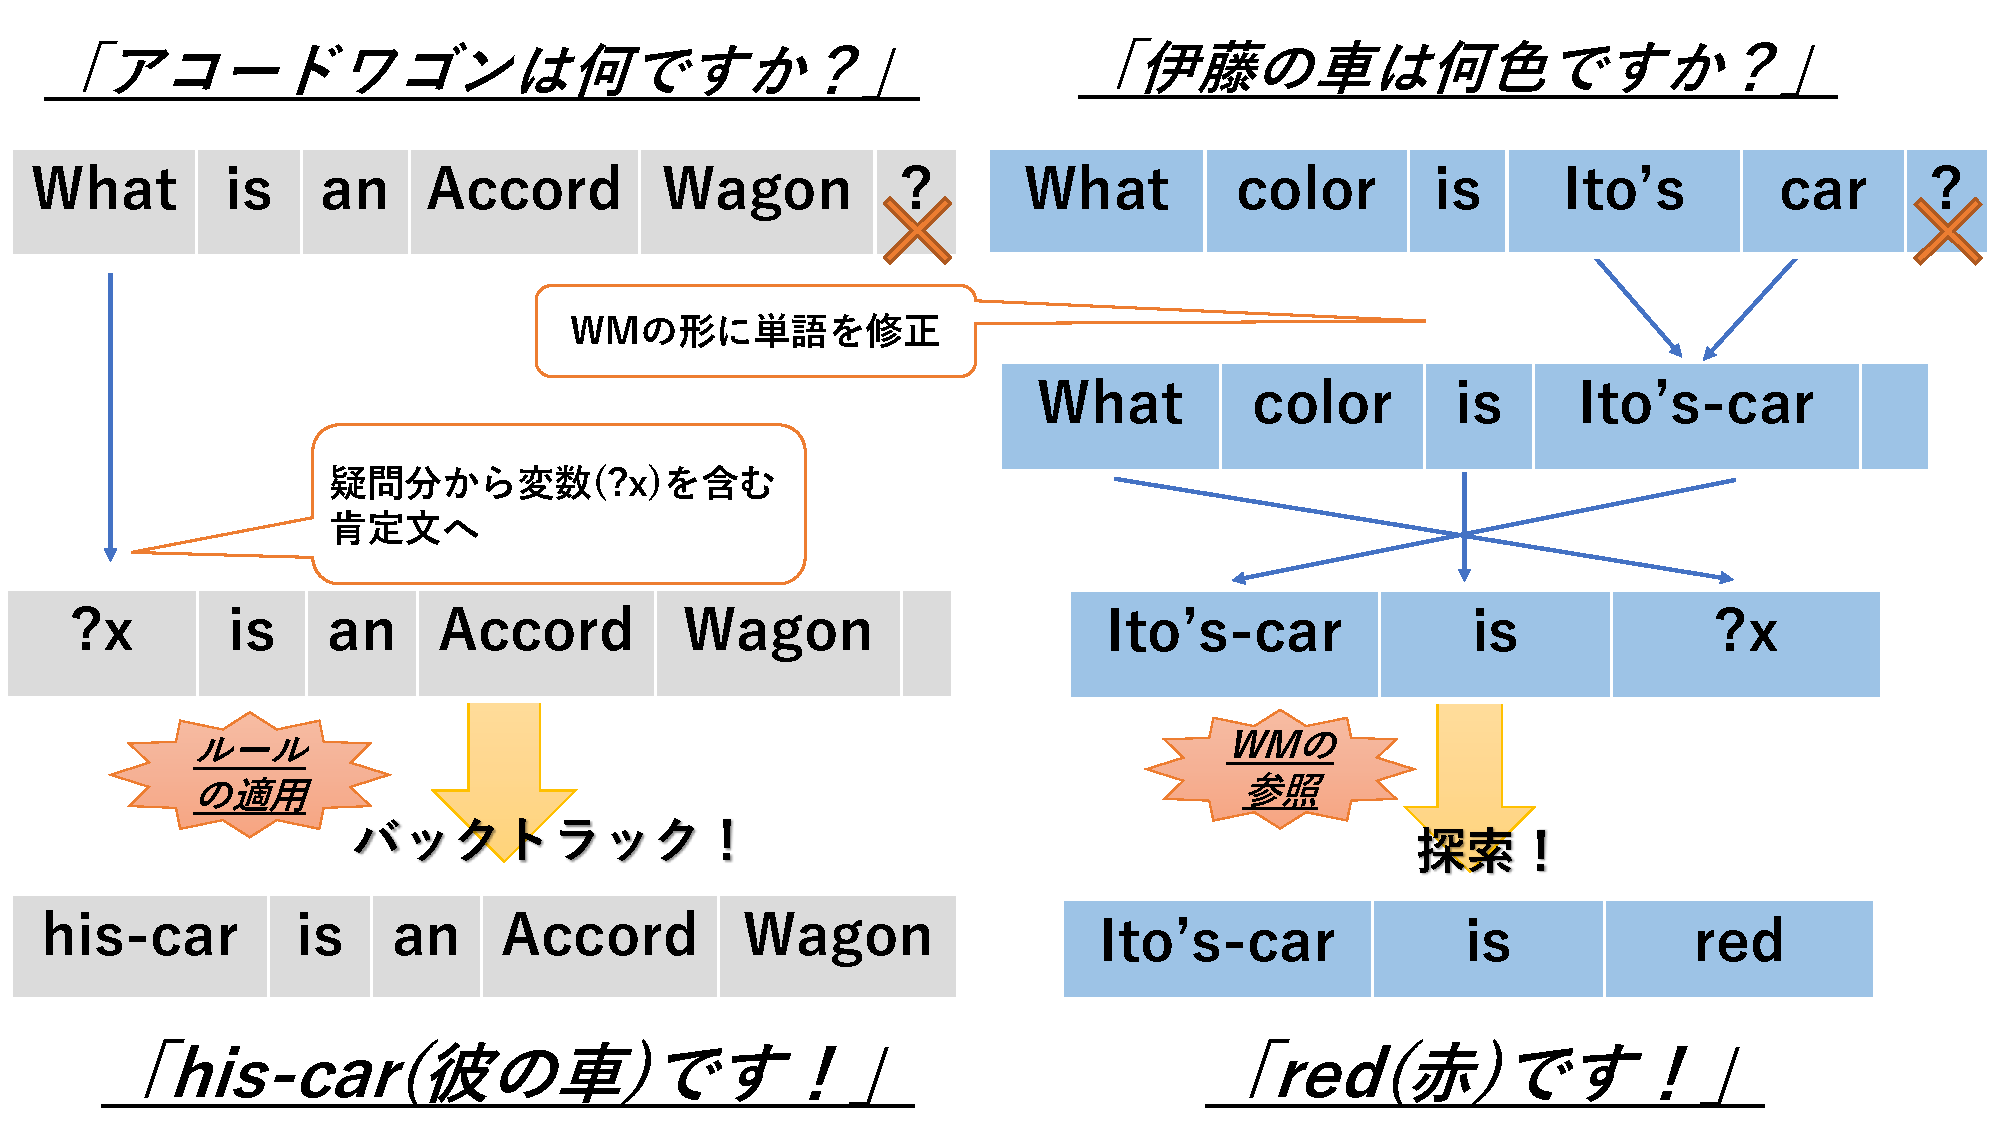
\includegraphics[width = 10cm, pagebox = cropbox, clip]{images/英文構造_疑問詞SVO.pdf}
 \end{center}
 \caption[]{具体的な答えを返す質問の処理}\label{fig:fig1.1}
\end{figure}

具体的な答えを返す質問, つまり, 質問文にWhatが含まれるもの対しては, 疑問分から肯定文に変換する際に変数?xを適切な場所に配置する. 図4の左の質問は, ルールの後件部の内容なので, バックトラックが行われ, 右の質問ではワーキングメモリが参照される. どちらも変数が具体化され, 答えが出力される. ここで問題になってくるのは, 図4の左側の質問のような, 変数を入れた場合のルールの適用によるバックトラックシステムである. バックトラックを行うためには, ルールの後件部の内容でなければならず, それ以外では, バックトラックが行われない. つまり, 「?x is an Accord Wagon」は質問できても, 「his-car is ?x」は使えないと述べたこのレポートの一番始めの内容の問題が生じる. これはこの推論システムの欠点ともいえる.

\subsection{前向き推論に関して}
前向き推論では, ワーキングメモリのアサーション集合とルールにより生成される新たなアサーションを, ワーキングメモリに次々と格納していくので, 質問に答える時には, 質問内容と最終的に出来上がったワーキングメモリに格納されているアサーションを1つ1つ照らし合わせればよい.
質問の種類もYes/Noと答えるものと, 具体的な値を答える方法の2種類であり, 後ろ向き推論と同じ方法が使える. また, 前向き推論は, 最終的なワーキングメモリだけを参照することから, 後ろ向き推論のようなに, 質問がルールの後件部に当てはまるかどうかを考える必要もない.

\section{実装}
英語の質問を変数に含むパターンに変換し, 解析をするメソッドNaturalLanguageメソッドを作成. メイン文で入力された英語の質問(String型)に対して実行し, 答えを出力する. 英語の質問内容を変数を含むパターンに落とす流れは, 後ろ向き推論でも前向き推論でも内容は同じであるが, 後ろ向き推論では, 実際に推論を行うbackwardChainメソッドを最後に使うのに対し, 前向き推論では, 先にforwardChainメソッドを呼び出して推論を行ってから, NaturalLanguageメソッドを呼び出す.そのメソッドを機能ごとに分けて以下に示す.

\subsection{手法1}
まずは, NaturalLanguageメソッドの始めの処理をソースコード\ref{src:No1}に示す。
\begin{lstlisting}[caption=NaturalLanguageメソッドその1, label=src:No1]
    public static void NaturalLanguage(String equestion) {
    	/***
    	 *	1. "英語の質問:s"を"変数含むパターン"に置き換える
    	 *	2. その"変数を含むパターン"を解析する:rb.backwardChain()を実行
    	 */
    	//解
    	ArrayList<String> tokenList = new ArrayList<>();
    	//今どこを指しているか
    	int tokenPoint = 0;

    	//前処理
    	if(equestion.contains("'s c")) {
    		equestion = equestion.replace("'s c", "'s-C");
    	}
    	else if(equestion.contains("his")) {
    		equestion = equestion.replace("his c", "his-c");
    	}
	else if(equestion.contains("my")) {
		equestion = equestion.replace("my c", "my-c");
	}

    	//1.まずはトークンに分解して,
    	StringTokenizer stoken = new StringTokenizer(equestion);
    	//  トークンの数を保存
    	int tokenSize = stoken.countTokens() - 1;	//最後の?は除く!
\end{lstlisting}

NaturalLanguageメソッドでは, まず前処理として, 英文とアサーションの違いを直す. 「Ito's-Car」は「Ito's car」に分け, 「his-car」は「his car」に, 「my-car」は「my car」に分けている. その後, String型のアサーションをトークンに分解し, 1つのアサーションがいくつのトークンに分解できたかを保持しておく.\\

次に, NaturalLanguageメソッドの中間部, トークンの並び替えの処理をソースコード\ref{src:No2}に示す.
\begin{lstlisting}[caption=NaturalLanguageメソッドその2, label=src:No2]
    	//2.トークンの並び替え,
    	String firstToken = stoken.nextToken();
    	tokenPoint ++;
    	String secondToken = stoken.nextToken();
    	tokenPoint ++;
    	if(firstToken.equals("Is")) {
    		tokenList.add(secondToken);
    		tokenList.add("is");
    	}
    	else if(firstToken.equals("What")) {
    		rb.qFlag = 1;
    		if(secondToken.equals("color")) {
    			String thirdToken = stoken.nextToken();
    			tokenPoint ++;
    			tokenList.add(stoken.nextToken());
    			tokenPoint ++;
    			tokenList.add(thirdToken);
    			tokenList.add(" ?x");
    		}
    		else if(secondToken.equals("does")) {
    			tokenList.add(stoken.nextToken());
    			tokenPoint ++;
    			String thirdToken = stoken.nextToken();
    			tokenPoint ++;
    			if(thirdToken.equals("have")) {
    				tokenList.add("has");
    			}
    			tokenList.add("?x");
    		}
    		else if(secondToken.equals("is")) {
    			tokenList.add("?x");
    			tokenList.add("is");
    		}
    	}
    	else if(firstToken.equals("Does")) {
    		String thirdToken = stoken.nextToken();
    		tokenPoint ++;
    		//三単現のs
    		if(thirdToken.equals("have")) {
    		  thirdToken = "has";
    		}
    		else {
    		  thirdToken = thirdToken.replace(thirdToken, thirdToken+"s");
    		}
    		tokenList.add(secondToken);
    		tokenList.add(thirdToken);
    	}
\end{lstlisting}

質問文ははじめのトークンが何かで大きく分岐できる. Whatで始まれば"具体的な値を問う質問"であり, Isで始まれば"Yes/No返事の質問"のSVC型, Doesで始まれば"Yes/No返事の質問"のSVO型となる. もちろんWhatのあとで, 同様に"is"と"does"で分けられる. 今回, 分解したトークンのどこを指しているかをint型のtokenPointで保存しておく. これは, 以下で述べられる最後の処理をする際に用いられる. \\

最後に, NaturalLanguageメソッドの最終部の処理を示す. ここは, 後ろ向き推論と前向き推論で異なる点があるので, まずは後ろ向き推論に関して, ソースコード\ref{src:No3}に示す.
\begin{lstlisting}[caption=NaturalLanguageメソッドその3(後ろ向き推論の場合), label=src:No3]
    	//3.toStringで最後に合体させる(今回はあくまでStrigの文字列にする.)
    	//  格納
    	for(int i = tokenPoint; i < tokenSize; i++) {
    		tokenList.add(stoken.nextToken());
    	}
    	//  ArrayList → String文字へ
    	String patarn = tokenList.toString();
    	patarn = patarn.replace("[", "");
    	patarn = patarn.replace("]", "");
    	patarn = patarn.replace(",", "");
    	System.out.println("patarn = " + patarn);

    	//解析
	    StringTokenizer patarns = new StringTokenizer(patarn,",");
	    ArrayList<String> queries = new ArrayList<String>();
	    for(int i = 0 ; i < patarns.countTokens();){
	    	queries.add(patarns.nextToken());
	    	System.out.println("queries = " + queries);
	    }
	    rb.backwardChain(queries);	//ここのqueriesはStringの文字列
    }
\end{lstlisting}

今回は, 前回のSemanticNetプログラムのように, Tail, Lavel, Headの3つに分けて当てはめるのではなく, 1つのString文として解析をするので, 分解してトークンを1つのString文にもどす必要がある. tokenListに各トークンを格納していくが, ソースコード1,2で述べた現在のトークンの位置を保存するtokenPointを用い, まだtokenListに代入されていない残りのトークンを代入する. Listを1つのStringにするには, toStringメソッドとリストに表現される"[かぎかっこ]"と",区切り文字"を取り除くことで実現している.\\

次に, NaturalLanguageメソッドの最終部の処理の前向き推論に関して, 後ろ向き推論と異なる箇所をソースコード\ref{src:No4}に示す.
\begin{lstlisting}[caption=NaturalLanguageメソッドその3(前向き推論の場合), label=src:No4]
   /*(注意)
     *	Yes/No返事のときは, そのままでいいんだけど,
     *  「my-car has ?x」のときに, 「?x= a VTEC engine」とかで複数トークンになる
     *  ので, Whatの場合は別にしないといけない
     */

  //whatに質問
  if(patarn.contains("?x")) {

	ArrayList<String> newWorkingMemory = new ArrayList<>();

	for(int i = 0; i < rb.wm.memorySize(); i ++) {
	    ArrayList<String> newAssertion = new ArrayList<>();
	    StringTokenizer wmtoken = new StringTokenizer(rb.wm.getValue(i));

	    String wmfirstToken = wmtoken.nextToken();
	    newAssertion.add(wmfirstToken);

	    String wmsecondToken = wmtoken.nextToken();
	    String wmthirdToken = wmtoken.nextToken();
	    if(wmsecondToken.equals("is") && wmthirdToken.equals("a")) {
	    	  newAssertion.add("is-a");
	    }
	    else if(wmsecondToken.equals("is") && wmthirdToken.equals("an")) {
	        newAssertion.add("is-an");
	    }
	    else if(wmsecondToken.equals("has") && wmthirdToken.equals("a")) {
		  newAssertion.add("has-a");
	    }
	    else if(wmsecondToken.equals("has") && wmthirdToken.equals("an")) {
		  newAssertion.add("has-an");
	    }
	    else if(wmthirdToken.equals("several")) {
		  newAssertion.add(wmsecondToken);
	    }
	    else {
		  newAssertion.add(wmsecondToken);
		  newAssertion.add(wmthirdToken);
	    }
	    //System.out.println("残りトークンの数 = " + wmtoken.countTokens());
	    if(wmtoken.countTokens() > 1) {
		   String wmforthToken = wmtoken.nextToken();
		   String wmfifthToken = wmtoken.nextToken();
		   newAssertion.add(wmforthToken + "-" + wmfifthToken);
	    }
	    else if(wmtoken.countTokens() == 1){
		   newAssertion.add(wmtoken.nextToken());
	    }
	    //System.out.println("newAssertion = " + newAssertion);
	    //  ArrayList → String文字へ
	    String stringAssertion = newAssertion.toString();
	    stringAssertion = stringAssertion.replace("[", "");
	    stringAssertion = stringAssertion.replace("]", "");
	    stringAssertion = stringAssertion.replace(",", "");
	    //System.out.println("stringAssertion = " + stringAssertion);
	    newWorkingMemory.add(stringAssertion);
			
	    //ystem.out.println("newWorkingMemory = " + newWorkingMemory);
	    //解析
	    for(int i = 0; i < newWorkingMemory.size(); i++) {
		   (new Matcher()).matching(patarn, newWorkingMemory.get(i));
	    }
	}

    //Yes/Noで答える質問
    else {
	    //解析
	    boolean flag = false;
	    for(int i = 0; i < rb.wm.memorySize(); i ++) {
		  if((new Matcher()).matching(patarn, rb.wm.getValue(i))) {
			 System.out.println("答え = Yes");
				flag = true;
		  }
	    }
	    if(!flag) {
		   System.out.println("答え = No");
	    }
    }
\end{lstlisting}
前向き推論では, リスト化されたワーキングメモリ内のアサーションを1つずつ検索していき, Matcherクラスのmatchingメソッドを呼び出すことで答えを出力させている. ただし, ここで"Whatで聞かれた具体的な値を返す質問"と"Yes/Noで返す質問"で大きな違いが生じる. Whatで聞かれた質問, つまり, 変数(?x)をマッチングで具体化させるとき, これまでのmatchingメソッドと同様に, 1つのトークン単位で行っているので, \\「?x = a VTEC engine」のような, 複数のトークンをまとめて出力させることはできない. なぜ"Yes/Noで答える質問"ではそれが生じないのかというと, Yes/Noではすでにトークンが指定数存在するからである. 以下をみてもらいたい.\\

(具体例)\\
肯定文の場合, \\
「my car has a VTEC engine.」\\
Yes/Noで返す場合の質問の場合,\\ 
「Does my car have a VTEC engine ?」  →  「my car has a VTEC engine」と変換可能\\
疑問文の場合,\\
「What does my car have ?」  →  「my car have ?x」としか変換できない...\\

そのため, 「VTEC engine」のような2つのトークンにまたがるものは, 1つにまとめないといけない. その時に, 「has」と「a」は「has-a」のようにまとめ, 「several」といいた複数の意味をもつ前置詞は取り除いている.

\section{実行例}

\subsection{後ろ向き推論:その1}
後ろ向き推論システムにおいて, 日本語で言うと, 「彼の車はアコードワゴンですか?」と質問したときの実行結果が以下のようになる.
\begin{lstlisting}
質問を入力してください
Is his-car an Accord Wagon ?
質問内容 = Is his-car an Accord Wagon ?
patarn = his-car is an Accord Wagon
queries = [his-car is an Accord Wagon]
Hypothesis:[his-car is an Accord Wagon]
Success RULE
Rule:CarRule11 [?x40 is a Honda, ?x40 is stylish, ?x40 has several color models, ?x40 has several seats, ?x40 is a wagon]->?x40 is an Accord Wagon <=> his-car is an Accord Wagon
Success RULE
Rule:CarRule7 [?x47 is made in Japan, ?x47 has Honda's logo]->?x47 is a Honda <=> ?x40 is a Honda
Success RULE
Rule:CarRule1 [?x48 is inexpensive]->?x48 is made in Japan <=> ?x47 is made in Japan
Success WM
his-car is inexpensive <=> ?x48 is inexpensive
tmpPoint: 13
Success:?x47 is made in Japan
tmpPoint: -1
Success RULE
Rule:CarRule8 [?x66 is made in Japan, ?x66 has a VTEC engine]->?x66 is a Honda <=> ?x40 is a Honda
Success RULE
Rule:CarRule1 [?x67 is inexpensive]->?x67 is made in Japan <=> ?x66 is made in Japan
Success WM
his-car is inexpensive <=> ?x67 is inexpensive
tmpPoint: 13
Success:?x66 is made in Japan
Success WM
his-car has a VTEC engine <=> ?x66 has a VTEC engine
tmpPoint: 20
Success:?x40 is a Honda
Success WM
his-car is stylish <=> ?x40 is stylish
tmpPoint: 3
Success:?x40 is stylish
Success WM
his-car has several color models <=> ?x40 has several color models
tmpPoint: 4
Success:?x40 has several color models
Success WM
his-car has several seats <=> ?x40 has several seats
tmpPoint: 5
Success:?x40 has several seats
Success WM
his-car is a wagon <=> ?x40 is a wagon
qFlag = 0
Yes
\end{lstlisting}

この質問内容はルールの後件部の内容に関わるので, バックトラックが行われていることがわかる. 結果正しく出力されていることが確認できる.

\subsection{後ろ向き推論:その2}
後ろ向き推論において, 日本語で言うと, 「伊藤の車は赤いですか?」と質問したときの実行結果が以下のようになる.
\begin{lstlisting}
Is Ito's car red ?
質問内容 = Is Ito's car red ?
patarn = Ito's-Car is red
queries = [Ito's-Car is red]
Hypothesis:[Ito's-Car is red]
Success WM
Ito's-Car is red <=> Ito's-Car is red
qFlag = 0
Yes
\end{lstlisting}

この質問内容はルールの後件部には存在しないので, ワーキングメモリだけが参照されていることがわかる. その結果, 正しく出力されていることがわかる.

\subsection{前向き推論:その1}
前向き推論において, 日本語で言うと,「私の車は何を持っていますか」と質問したときの実行結果が以下のようになる.
\begin{lstlisting}
質問を入力してください
What does my car have ?
質問内容 = What does my car have ?
patarn = my-car has ?x
newWorkingMemory = [my-car is inexpensive, my-car has-a VTEC-engine, my-car is stylish, my-car has color-models, my-car has seats, my-car is-a wagon, my-car is made in-Japan, my-car is-a Honda, my-car is-an Accord-Wagon]
答え = color-models
答え = seats
\end{lstlisting}
英語の質問文が, 変数を含むパターンに正しく変換された後, 「has-a」や「VTEC-engine」など通常のワーキングメモリから改良した新しいワーキングメモリが生成され, それにより正しい答えが出力されている. 後ろ向き推論とは異なり, リスト構造のワーキングメモリを1つずつ参照しているだけなので, 複数の回答の出力も容易に実現されていることがわかる. 

\subsection{前向き推論:その2}
前向き推論において, 日本語で言うと,「私の車はVTECエンジンを持っていますか」と質問したときの実行結果が以下のようになる.
\begin{lstlisting}
質問を入力してください
Does my car have a VTEC engine ?
質問内容 = Does my car have a VTEC engine ?
secondToken = my-car
patarn = my-car has a VTEC engine
答え = Yes
\end{lstlisting}
「前向き推論:その1」の実行結果とは異なり, 新しいワーキングメモリを作成する必要がないので, そのまま出力させている. 正しくYesの答えが返ってきていることが確認できる.

\subsection{CupNoodle.dataに基づく推論システム}
小中君が考えてくれた, CupNoodleのルール(CupNoodle.data)と, ワーキングメモリ(CupNoodleWm.data)を用いて, 英語による質問応答システムを実行してみる.

\subsubsection{前向き推論}


\section{考察}
今回は前向き推論と後ろ向き推論において, 同じ質問内容でも, その推論システムの機能の違いから, 違うアプローチが必要になることがわかった. 後ろ向き推論における質問の内容には大きく4パターンに分けることができた. 以下を参考にしてもらいたい.

\begin{figure}[htbp]
 \begin{center}
  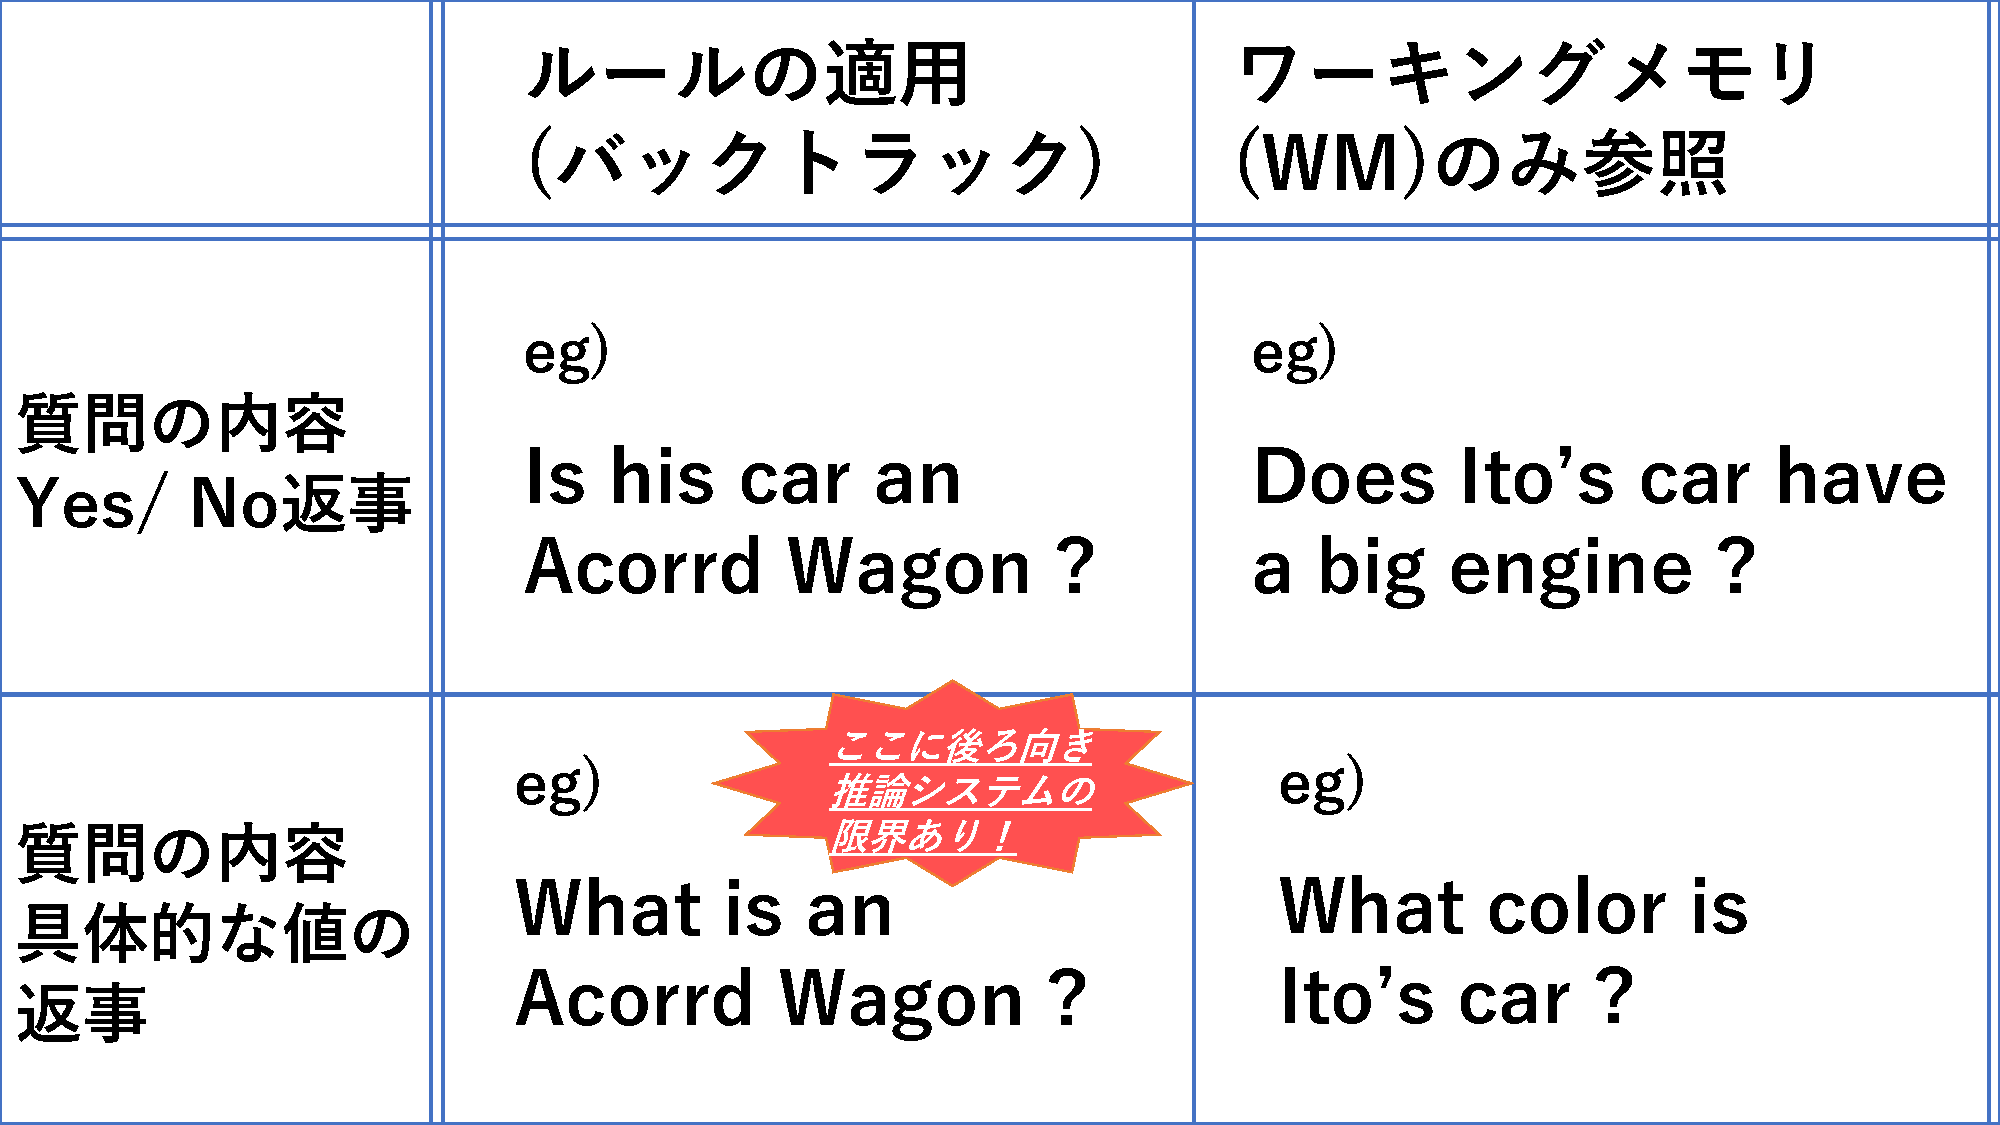
\includegraphics[width = 8cm, pagebox = cropbox, clip]{images/後ろ向き推論の質問の分類.pdf}
 \end{center}
 \caption[]{後ろ向き推論の質問の分類}\label{fig:fig1.1}
\end{figure}

これまでさんざん述べてきたように, 後ろ向き推論が仮説を検証することにおいて, 全ての文章に対応していない. あくまで, 仮説にできる内容はルールの後件部の内容であり, それ以外はワーキングメモリを参照するだけである.

また, 今回の自分のように, 英語の質問文をトークンに分けて処理する流れだと, 「?x = a VTEC engine」のような複数のトークンにまたがってしまう答えに応えることがとても大変になってしまった. 実際に前向き推論では新しくワーキングメモリを作らざるを得なくなり, 後ろ向き推論に当たってはうまく答えを出力できていない状態である.

\section{感想}
人間の認識システムをプログラムに落としこんだとされるルールベースモデルにおける後ろ向き推論システム, これにおいて, 検証できる仮説の内容が限定さえれてしまうことに驚きを隠せない. 自分の質問のさせ型に全く別のアプローチを用いるか, 新たな知識(ルール)を構築させることで, この現状を打破できるのかどうかについては今後に期待していきたい. 

また, 2つの課題にわたり英語の自然言語を扱ってきたが, 今回のトークンの問題のようにまだまだ再現性が低い状態が続いた. 英語でこの大変さなので, 日本語にいたっては, いくら時間を使っても足りないであろうと感じた. 大量のコーパスを用い, 研究を進める自然言語学者は本当に大変な研究をしていると思った.

%%%%%%%%%%%%%%%%%%%%%%%%%%%%%%%%%%%%%%%%%%%%%%%%%%%%%%%%%%%%%%%%%%%%%%%%%%%%%%
% 参考文献
\begin{thebibliography}{99}
\bibitem{notty} Javaによる知能プログラミング入門 --著:新谷 虎松 \\
\bibitem{notty} HashMap --著:Java コード入門 \\
\url{http://java-code.jp/232}
\bibitem{notty} Google翻訳 --著:Google \\
\url{https://translate.google.com/?hl=ja}
\bibitem{notty} java substringメソッド --著:Engineer.club \\
\url{https://engineer-club.jp/java-substring}
\end{thebibliography}
\end{document}